\documentclass[10pt,twocolumn,journal]{IEEEtran}
% XeLaTeX: all fonts are resolved from the local installation.
\usepackage{fontspec}
\defaultfontfeatures{Ligatures=TeX}
\setmainfont[
  BoldFont=TeXGyreTermes-Bold,
  ItalicFont=TeXGyreTermes-Italic,
  BoldItalicFont=TeXGyreTermes-BoldItalic,
  SmallCapsFont=TeXGyreTermes-Regular,
  SmallCapsFeatures={Letters=SmallCaps}
]{TeXGyreTermes-Regular}
\IfFontExistsTF{Arial}{\setsansfont{Arial}}{\setsansfont{Liberation Sans}}
\setmonofont{TeXGyreCursor-Regular}

\usepackage[margin=1in,bottom=1in]{geometry}
% Normal line spacing; content hierarchy provides the space savings.
\setlength{\textfloatsep}{10pt plus 2pt minus 2pt}
\setlength{\dbltextfloatsep}{10pt plus 2pt minus 2pt}
\setlength{\floatsep}{7pt plus 2pt minus 2pt}
\setlength{\abovecaptionskip}{4pt}
\usepackage{amsmath,amssymb}
\usepackage{booktabs,array}
\usepackage{graphicx}
\usepackage{xr-hyper}
\usepackage[hidelinks]{hyperref}
\usepackage{fancyhdr}
\graphicspath{{figures/}}
\setcounter{equation}{13}
\setcounter{table}{4}
\setcounter{figure}{4}
\setlength{\emergencystretch}{2em}
\renewcommand{\topfraction}{0.95}
\renewcommand{\dbltopfraction}{0.95}
\renewcommand{\textfraction}{0.05}
\renewcommand{\floatpagefraction}{0.85}
\renewcommand{\dblfloatpagefraction}{0.85}
\setcounter{topnumber}{3}
\setcounter{dbltopnumber}{3}
\pagestyle{fancy}
\fancyhf{}
\fancyhead[L]{\scriptsize BELOW ZERO --- SUPPLEMENTARY MATERIAL}
\fancyhead[R]{\scriptsize\thepage}
\renewcommand{\headrulewidth}{0pt}
\externaldocument{main}[main.pdf]
\makeatletter\setlength{\@fptop}{0pt}\setlength{\@fpsep}{16pt}\setlength{\@fpbot}{0pt plus 1fil}\makeatother
\newcommand{\BZAuthorBlockEN}{Yaogeng Jiang\\Independent Researcher\\\href{mailto:y.g.jiang@sjtu.edu.cn}{y.g.jiang@sjtu.edu.cn}}
\newcommand{\BZAuthorBlockZH}{姜尧耕\\独立研究者\\\href{mailto:y.g.jiang@sjtu.edu.cn}{y.g.jiang@sjtu.edu.cn}}
\newcommand{\BZPDFAuthors}{Yaogeng Jiang}

\hypersetup{pdfauthor={\BZPDFAuthors}}
\begin{document}
\title{Below Zero: Supplementary Material}
\author{\BZAuthorBlockEN}
\maketitle
\thispagestyle{fancy}

This supplement provides derivation notes, implementation details, regional and calibration analyses, and development-set controls. Numbering continues from the main text, and full-precision scores and source-image identifiers are included in the accompanying archive.

\section{Units, Conditioning, and the Meaning of a Sample}
\subsection{Signal Versus Readout}
The network output $s\geq0$ represents the expected signal in DN, with corresponding photoelectron mean $s/g$. With $N\sim\operatorname{Poisson}(s/g)$, the forward simulator's integer path is
\begin{equation}
\begin{aligned}
A&=\min\{16383,\lfloor512+gN+\epsilon+b+1/2\rfloor\},\\
V&=A-512.
\end{aligned}
\end{equation}
All simulated realizations remain above the physical lower bound of the ADC. The four CFA-phase offsets are drawn independently and uniformly over $[-0.25,0.25]$ DN per realization and enter both the estimator and the decoder as known conditions.

At a censored pixel, observing $Y_i=0$ implies $V_i\leq0$. Under independent sensor noise, neighboring measurements inform the latent signal $s_i$, while the conditional law evaluated at the estimated signal specifies the missing readout distribution.

Let $m=\mathbb E[V\mid Y,s]$ and $v=\operatorname{Var}(V\mid Y,s)$ at a censored pixel. For an independent draw $V'$ from the same conditional law,
\begin{align}
\mathbb E[(V-m)^2\mid Y,s]&=v,\\
\mathbb E[(V-V')^2\mid Y,s]&=2v.
\end{align}
A squared-error criterion therefore favors the conditional mean $m$, which suppresses variation, over a statistically faithful draw $V'$. This motivates the proper distribution scores used in the main comparison.

\subsection{Excess Scores and the Known-Signal Reference}
For the known-signal conditional law $p_i^\star$ and a predicted distribution $q_i$ on a common discrete support,
\begin{equation}
\mathbb E_{V\sim p_i^\star}[-\log q_i(V)]-H(p_i^\star)=D_{\mathrm{KL}}(p_i^\star\|q_i).
\end{equation}
For the ranked probability score, expanding the squares gives
\begin{equation}
\begin{split}
&\mathbb E_{V\sim p_i^\star}[\operatorname{CRPS}(q_i,V)-\operatorname{CRPS}(p_i^\star,V)]\\
&\qquad=\Delta\sum_k\left(F_{q_i}(k)-F_{p_i^\star}(k)\right)^2.
\end{split}
\end{equation}
These identities separate conditional readout uncertainty from distribution-estimation error, since the known-signal law has zero self-divergence and zero cumulative discrepancy while its realized NLL remains nonzero. For a negative label $V<0$, deterministic zero fill has ranked score $|V|$ and infinite NLL, which the main table reports directly.

\section{Network, Data, and Training Details}
\subsection{Network Architecture}
We pack the Bayer phases as $[R,G_1,G_2,B]$ and provide 16 input channels comprising four $\operatorname{asinh}(Y/4)$ measurements, four zero-candidate indicators, four broadcast offset maps, a validity mask, and three constant maps for $g$, $\sigma_r$, and a reserved zero. The validity mask distinguishes padded border pixels from measured zeros, while the known offsets enter both the estimator and the PG decoder.

Table~\ref{tab:architecture} summarizes the NAF-style architecture. Each normalization operates across channels at one spatial location in FP32 arithmetic with $\epsilon=10^{-6}$. SimpleGate multiplies two channel halves, and learned residual scales are initialized to zero.

\begin{table}[t]
\centering
\caption{N0 architecture in packed CFA coordinates.}
\label{tab:architecture}
\footnotesize
\setlength{\tabcolsep}{3pt}
\begin{tabular}{@{}lccc@{}}
\toprule
Stage & Width & Blocks & Spatial scale\\
\midrule
Input stem & 32 & --- & 1\\
Encoder 1 & 32 & 2 & 1\\
Encoder 2 & 64 & 2 & 1/2\\
Encoder 3 & 128 & 4 & 1/4\\
Encoder 4 & 256 & 4 & 1/8\\
Bottleneck & 512 & 4 & 1/16\\
Decoder 1--4 & 256/128/64/32 & 2 each & 1/8 to 1\\
Signal head & 4 & --- & 1\\
\bottomrule
\end{tabular}

\vspace{3pt}
\footnotesize The 16 input channels comprise 4 transformed measurements, 4 zero indicators, 4 offset maps, 1 validity mask, and 3 constant maps, and the output consists of 4 softplus signal maps. The 10,913,380-parameter model uses no pooled channel or spatial attention.
\end{table}

Nested 128- and 256-pixel contexts share a central 64-pixel target, even Bayer alignment, and boundary validity masking, with geometric flips and rotations applied prior to packing.

\subsection{Synthetic Distribution and Split Integrity}
In the calibrated profile, the measured integer-domain read-noise variance is reduced by $1/12\,\mathrm{DN}^2$ before the explicit 1-DN quantizer is applied in simulation.

The 1,100 rendered RGB templates are split into 825 training, 137 development, and 138 test sources. Natural draws (90\%) use median-normalized log-uniform exposure over 0.4--64 DN and color multipliers $\exp U[-0.3,0.3]$, where 30\% add a 0.1--2 DN dark floor, 5\% are zero-light controls, and procedural draws supply the remaining 10\%. All synthetic settings are independent of the real exposures.

Each test source has two cases with independent crop, augmentation, exposure, and noise seeds. All estimators evaluate each case, and both contexts share its center, while bootstrap resampling keeps all four conditions of a source together.

\subsection{Optimization and Precision}
AdamW uses a $2\times10^{-4}$ peak learning rate, a 2,000-update warmup, cosine decay to $2\times10^{-6}$ at 80,000 updates, weight decay of 0.01, gradient clipping at 1, and moving-average (EMA) decay of 0.999. Two physical batches of size one are accumulated per update, each contributing at most 2,048 zero candidates to the conditional cross-entropy loss. Evaluations use the EMA checkpoint at update 80,000 of seed 7103.

The physical decoder evaluates 306 category probabilities from the four predicted signal maps. Training uses mixed precision, whereas final network inference uses FP32 with TF32 disabled, and likelihood and mixture integrations use FP64 where required.

\subsection{Score Aggregation and Confidence Intervals}\label{sec:scoreaggregation}
Candidate scores are averaged within each case, across nonempty cases within each source, and then across sources with equal weight. Paired bootstrap resampling treats a source and all of its cases as one unit, using 10,000 resamples for aggregate comparisons. The preregistered KL contrasts against Local Bayes and Foi-qPG use 97.5\% percentile intervals (controlling the familywise error rate at 5\% across both tests), while secondary comparisons use 95\% intervals. Regional comparisons are exploratory and follow the pointwise 95\% procedure in Section~\ref{sec:regionaldefinitions}, without multiplicity adjustment for development or regional slices. All intervals condition on the trained model and quantify source-image sampling variability.

\section{Tail Resolution and Probability Calibration}
The lookup table (LUT) uses steps of 0.002 in $\log(1+s)$ and 0.01 DN in $b$. Across 152 archived validation queries, the maximum teacher-to-interpolant KL divergence is $2.18\times10^{-7}$ nats and the maximum mass-normalization error is $7.77\times10^{-16}$.

\subsection{Resolving Codes Within the Tail}
Let $K=304$ and $T=\{V<-K\}$. The stored LUT law is
\begin{equation}
\bar q=(q(0),q(-1),\ldots,q(-K),q(T)).
\end{equation}
Excess KL compares the normalized coarsened laws $\bar p^\star$ and $\bar q$, accounting for the total tail mass in $T$ without distinguishing distributions within $T$.

Whenever category $T$ is selected during sampling, a second independent coordinate-seeded substream draws an integer from the PG law conditional on $T$. For a withheld tail code $k<-K$, the resolved log probability is
\begin{equation}
\log q(k)=\log q(T)+\log p_{\mathrm{PG}}(k)-\log P_{\mathrm{PG}}(T).
\end{equation}
For Bayesian mixtures, this evaluation retains every signal component's tail law and posterior weight, since substituting a single mean signal would alter the tail distribution.

Truncation residuals for the conditional moments and ranked-score calculations are below $10^{-12}$. A $-400$ DN test verifies mixture-tail evaluation against independent scalar laws, and real tail labels are evaluated at their actual integer codes.

\subsection{Calibration Versus Sampler Verification}
Table~\ref{tab:coverage} reports discrete interval calibration on the fixed 32-source development cohort, comparing empirical coverage with each equal-tail interval's actual predicted probability mass.

\begin{table}[t]
\centering
\caption{Discrete-interval calibration on 32 development sources. Predicted and observed values are percentages. Difference is observed coverage minus actual predicted interval mass, in percentage points.}
\label{tab:coverage}
\footnotesize
\setlength{\tabcolsep}{3pt}
\begin{tabular}{@{}lrrrr@{}}
\toprule
Method & Nominal & Predicted & Observed & Difference\\
\midrule
N0/PG & 50\% & 52.584 & 52.460 & $-0.123$\\
N0/PG & 80\% & 81.864 & 81.510 & $-0.354$\\
N0/PG & 90\% & 91.819 & 91.685 & $-0.134$\\
N0/PG & 95\% & 97.632 & 97.597 & $-0.035$\\
Local PG & 50\% & 52.177 & 51.962 & $-0.215$\\
Local PG & 80\% & 81.981 & 81.509 & $-0.472$\\
Local PG & 90\% & 91.929 & 91.658 & $-0.270$\\
Local PG & 95\% & 97.639 & 97.538 & $-0.101$\\
Known signal & 50\% & 52.496 & 52.378 & $-0.118$\\
Known signal & 80\% & 81.864 & 81.513 & $-0.352$\\
Known signal & 90\% & 91.854 & 91.725 & $-0.129$\\
Known signal & 95\% & 97.635 & 97.601 & $-0.034$\\
\bottomrule
\end{tabular}
\end{table}

With fixed predicted laws and coordinate keys, reversing pixel order or processing candidates in chunks of size 257 leaves the sampled output unchanged. All outputs preserve positive codes, fill zero candidates with nonpositive integers, and reproduce the input after clipping.

Across 2,048 fixed predicted laws with two random streams and $S\in\{1,8,32,64\}$ draws (reference RMSE $\sqrt{\operatorname{Var}/S}$), sample-mean RMSE drops from 15.164 DN at one draw to 1.949 DN at 64 draws, tracking $S^{-1/2}$ scaling. At 64 draws, the mean per-location sample variance is 227.397 DN$^2$, matching the 226.970 DN$^2$ analytical prediction, with both streams included in the archived curve.

\section{Input Information and Additional Spatial Analyses}
\subsection{Local Likelihood and Bayesian Integration}
For each same-CFA neighborhood $\mathcal N_i$, let $h_{it}$ be the count of observed code $t$. The local signal log-likelihood is
\begin{equation}
\ell_i(s)=h_{i0}\log c(s,b)+\sum_{t>0}h_{it}\log p_Y(t\mid s,b).
\end{equation}
Upper saturation contributes a discrete event mass. Local PG refines a grid maximum of $\ell_i(s)$, whereas Local Bayes integrates the conditional laws against the training-fitted zero-plus-Gamma signal prior, with the center event counted once in both. The signal grid uses approximately 0.1 DN spacing below 32 DN and 0.5 DN above, converted to photoelectron means by $g$.

N0 uses four-phase multiscale context, whereas Local PG, Local Bayes, and Foi-qPG use same-phase observations. Joint-CFA Bayes (Section~\ref{sec:v3}) combines four-phase observations in a $5\times5$ window with a finite empirical prior.

\subsection{Held-Out Regional Definitions}\label{sec:regionaldefinitions}
Regional stratification of the held-out set uses same-CFA $9\times9$ neighborhoods. With $u=\log(1+s)$, local signal variation is $t=\sqrt{\overline{u^2}-\bar u^2}$ over valid pixels. Thresholded gradient locations have Sobel magnitude on $u$ of at least 0.15 after division by eight and a one-pixel validity erosion. Edge distance is Euclidean in packed pixels, and the zero fraction $z$ is the valid-neighborhood mean of $\mathbf1[Y=0]$.

Bin edges are $0,.25,.5,1,2,4,8,16,\infty$ DN for signal, $0,.025,.05,.1,.2,.4,.8,\infty$ for variation, $0,1,2,4,8,16,\infty$ for edge distance, and $0,.1,.25,.5,.75,.9,1$ for zero fraction, partitioning 1,627,306 unique candidates in the 256-pixel context. For each source and bin, we divide the combined score sum across both cases by their combined candidate count and then average available sources equally. Pointwise 95\% intervals use 2,000 paired source resamples (seed 1280027). Contributing source counts vary by bin (e.g., $z\geq0.75$ has two candidates from one source), and all counts and scores are archived in \texttt{V9\_heldout\_spatial\_bins\_256.csv}.

In the boundary bin $s<0.25$ DN (311,545 candidates from 94 sources), N0 minus Foi-qPG excess KL is $5.35\times10^{-5}$ nats (interval $[2.68,9.88]\times10^{-5}$), and N0 minus Local Bayes is $-8.72\times10^{-5}$ nats ($[-25.0,0.693]\times10^{-5}$), showing that uniform near-black regions differ from structured regimes.

\subsection{Development Absolute Errors and Matched Contrasts}
Fig.~\ref{fig:absolutegradient} reports absolute source-mean excess KL on the 32-source development set across low-, middle-, and high-gradient groups, where N0 and Local PG attain $0.000191$ vs.\ $0.000791$, $0.000249$ vs.\ $0.001007$, and $0.000442$ vs.\ $0.002109$ nats. From low to high gradient, the paired KL difference (N0 minus Local PG) changes by a mean of $-0.001066$ nats (median $-0.000102$, 23 of 32 sources negative, 10,000-resample interval $[-0.002177,-0.000271]$), with the two largest reductions contributing 65.7\% of the net sum, while the NLL contrast is $-0.000807$ nats ($[-0.003231,0.001221]$, 12 of 32 negative).

Coarse signal matching retains source--CFA--signal-bin cells with at least five low- and five high-gradient candidates, weighting cells by the smaller count within each source before averaging sources equally. Across 142 cells from 27 sources, the high-minus-low KL shift has mean $-0.000268$ nats (median $-0.0000358$, 18 of 27 negative, 20,000-resample interval $[-0.000581,-0.0000280]$), while the NLL shift is $0.000122$ nats ($[-0.002049,0.002086]$). Table~\ref{tab:adverse} lists regional NLL contrasts that favor a comparator or have intervals crossing zero.

\begin{figure}[t]
\centering
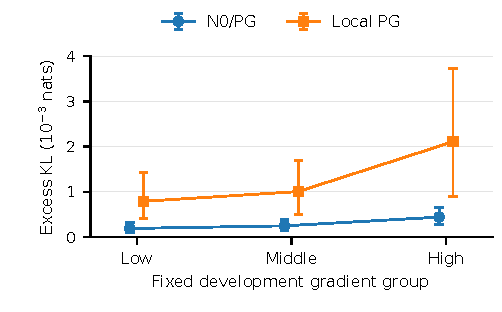
\includegraphics[width=\columnwidth]{s10_absolute_gradient.pdf}
\caption{Absolute conditional-distribution errors on the fixed 32-source development set. Points and 95\% source-bootstrap intervals use equal source weighting within each gradient group. Both errors rise with gradient, with Local PG rising more steeply. The cohort and grouping differ from the held-out marginal comparisons in Fig.~4 of the main text.}
\label{fig:absolutegradient}
\end{figure}

\begin{table*}[t]
\centering
\caption{Selected regional NLL contrasts that favor a comparator or have intervals crossing zero. N0-minus-comparator differences and pointwise 95\% source-bootstrap intervals are in $10^{-3}$ nats. The first two rows are post-hoc held-out case groups with zero fraction $z_{\mathrm{case}}\geq0.5$, while the remaining rows use development candidates. Here $d$ is the Sobel magnitude of $\log(1+s)$ divided by eight, and $a$ is the four-connected zero-component size in packed pixels.}
\label{tab:adverse}
\begin{tabular}{@{}llrrrr@{}}
\toprule
Feature / bin & Comparator & Sources & Difference & \multicolumn{2}{c}{95\% interval}\\
\midrule
Case zero fraction $\geq0.5$ & Local Bayes & 30 & $+0.0020$ & $-0.0132$ & $+0.0172$\\
Case zero fraction $\geq0.5$ & Foi-qPG & 30 & $+0.0080$ & $-0.0039$ & $+0.0200$\\
Signal $0\leq s<2$ DN & N0 permuted & 28 & $+1.3432$ & $-2.3007$ & $+6.1834$\\
Signal $s\geq16$ DN & Local PG & 20 & $-1.9514$ & $-4.0343$ & $+0.2155$\\
Gradient $0\leq d<0.025$ & Local PG & 32 & $+0.0043$ & $-1.4801$ & $+1.6993$\\
Gradient $0.025\leq d<0.1$ & Local PG & 32 & $+0.1099$ & $-0.9157$ & $+1.2081$\\
Gradient $d\geq0.1$ & Local PG & 32 & $-0.8031$ & $-2.0314$ & $+0.3147$\\
Zero-component size $a\geq33$ & Local PG & 30 & $-0.5950$ & $-2.0038$ & $+0.5810$\\
Zero-component size $a\geq33$ & N0 permuted & 30 & $-0.5265$ & $-3.8384$ & $+3.0659$\\
\bottomrule
\end{tabular}
\end{table*}

\subsection{Why Pooled Curves Can Overlap}
By the triangle inequality for total variation (TV) distance, spatially averaging distributions cancels opposite locationwise differences:
\begin{equation}
\operatorname{TV}\!\left(\frac1n\sum_iq_i,\frac1n\sum_ir_i\right)
\leq\frac1n\sum_i\operatorname{TV}(q_i,r_i).
\end{equation}
Development mean pointwise TV is 0.01235, whereas real pooled-PMF TVs drop to 0.000282 and 0.001561 across cohorts and weights. The archived pointwise histogram retains the full spread, while paired scores evaluate locationwise accuracy prior to pooling.

\section{Real-Exposure and Downstream Protocols}
\subsection{Integer Alignment and Hidden References}
\begin{table}[t]
\centering
\caption{Real-data NLL and CRPS differences under tail and repeated-coordinate exclusions, showing N0 minus Local PG on common R/$G_1$/$G_2$ candidates (negative values favor N0). The all-event row gives the full-sample result, followed by subsets selected using the retained readouts.}
\label{tab:real_robust}
\footnotesize
\setlength{\tabcolsep}{2.2pt}
\begin{tabular}{@{}llrrr@{}}
\toprule
Frame & Included positions & $N$ & $10^3\Delta$NLL & $\Delta$CRPS (DN)\\
\midrule
4748 & All & 12,652 & $-1.342$ & $-0.01102$\\
 & $V>-128$ & 12,609 & $-1.375$ & $-0.01145$\\
 & Excl. repeat coords. & 12,650 & $-1.336$ & $-0.01098$\\
\addlinespace[2pt]
4749 & All & 19,200 & $-0.964$ & $-0.00920$\\
 & $V>-128$ & 19,121 & $-0.998$ & $-0.00927$\\
 & Excl. repeat coords. & 19,198 & $-0.945$ & $-0.00907$\\
\bottomrule
\end{tabular}
\end{table}

Real references use the fixed integer shift $V=R_{\mathrm{native}}-512+n_c$, with $n_c=(2,3,3,3)$ DN for R/$G_1$/$G_2$/B, preserving the native quantization grid and camera files. Independent dark-frame calibration leaves fractional residuals of $(-0.437,-0.310,-0.189,+0.078)$ DN, and because zero inference offsets are supplied, these residuals remain part of the real-data model mismatch.

Table~\ref{tab:tail_original} reports the nested zero-atom and tail counts across all 31,852 shared R/$G_1$/$G_2$ candidates (including the fixed $-125$ DN diagnostic alongside the $-128$ DN threshold of Table~\ref{tab:real_robust}), while Section~\ref{sec:realcode} traces the deepest labels to their native codes.

\begin{table}[t]
\centering
\caption{Zero-atom and tail events among all 31,852 shared real R/$G_1$/$G_2$ candidates. Expected counts sum N0 probabilities, and observed counts use the retained signed labels.}
\label{tab:tail_original}
\begin{tabular}{@{}lrr@{}}
\toprule
Event & Expected count & Observed count\\
\midrule
$V=0$ & 1107.76 & 1190\\
$V\leq-1$ & 30744.24 & 30662\\
$V\leq-50$ & 1345.75 & 1065\\
$V\leq-125$ & 0.01690 & 132\\
$V\leq-305$ & $8.63\times10^{-30}$ & 13\\
\bottomrule
\end{tabular}
\end{table}

\subsection{Fixed Demosaicking Pipeline}
The fixed LibRaw 0.22.1 pipeline calls \texttt{open\_bayer(black=0)}, \texttt{unpack}, \texttt{raw2image\_ex(0)}, \texttt{pre\_interpolate}, and \texttt{ahd\_interpolate}, followed by FP32 pedestal subtraction, bypassing default black subtraction, scaling, white balance, color/gamma conversion, and denoising. Negative-pattern tests verify that below-black values reach interpolation, and the standalone build reproduces all six full-frame linear RGB arrays exactly. Because AHD's nonlinear decisions depend on the pedestal (verified at $P=512$ and $P=1024$), all comparisons evaluate $H(V+512)-512$.

\subsection{A/B/C/D Statistics}
Each real ROI is $512\times512$ Bayer pixels, leaving $480\times480$ evaluated RGB pixels after removing a 16-pixel border. Routes A and B are fixed signed and clipped references, while Routes C and D each demosaic 32 conditional draws separately and compute spatial statistics per draw before averaging. Route D uses the $3\times3$ Local PG window on real data ($5\times5$ on synthetic data).

\begin{table*}[t]
\centering
\caption{Linear camera-RGB statistics in the two preselected darkest real ROIs, before white balance or display clipping. Routes A and B are fixed references, while Routes C and D average the spatial statistics of 32 separately demosaicked samples. Units are DN. The data contain all 12 ROIs.}
\label{tab:ahd}
\begin{tabular}{@{}llrrrrr@{}}
\toprule
Exposure & AHD input & $\mu_R$ & $\mu_G$ & $\mu_B$ & sd$(R-G)$ & sd$(B-G)$\\
\midrule
P2654748 & A: signed reference & 8.041 & 9.003 & 3.200 & 25.986 & 22.037\\
& B: clipped & 15.368 & 16.322 & 11.707 & 18.635 & 15.127\\
& C: N0 samples & 7.924 & 8.621 & 1.655 & 25.157 & 22.495\\
& D: Local PG samples & 7.933 & 8.602 & 1.642 & 25.256 & 22.587\\
P2654749 & A: signed reference & 0.423 & 0.797 & $-0.225$ & 23.584 & 20.529\\
& B: clipped & 10.089 & 10.287 & 9.146 & 15.243 & 12.712\\
& C: N0 samples & 0.231 & 0.246 & $-1.871$ & 22.813 & 20.860\\
& D: Local PG samples & 0.352 & 0.352 & $-1.812$ & 22.799 & 20.861\\
\bottomrule
\end{tabular}
\end{table*}

Table~\ref{tab:ahd} reports the two preselected darkest ROIs. Intervals across draws describe completion sampling variation, while spatial standard deviations include scene texture and demosaicking correlation.

\subsection{Processing-Order Illustration}
\href{visual_en.pdf}{Supplementary Visual A} shows the P2654749 crop at $(0,1500)$ ($1000\times1000$ Bayer pixels, full-frame AHD, and fourfold area reduction to $250\times250$ pixels), where the routes share exposure and display transforms and differ only in RAW/RGB clipping order.

\subsection{Fixed Clean-Reference Color Endpoint}\label{sec:cleanendpoint}
This development protocol was locked before color scores were computed, with no preset perceptual threshold. Eight geometrically complete natural crops were selected from the 32-source development set without using endpoint scores (four procedural templates were evaluated separately). Each scene generated 16 independent PG realizations and two conditional draws per estimator and realization. The renderer used integer AHD at pedestal 512, fourfold signed-domain integration, fixed white balance and color matrix, and one clean-reference exposure per scene. Excluding border blocks, the eight darkest clean-reference blocks formed the evaluation region, scored by squared block-mean $(R-G,B-G)$ error in exposure-scaled linear display RGB against clean-$Q$-AHD, where $Q(s)=\lfloor s+0.5\rfloor$, and conditional means were quantized with the same $Q$ before AHD. Scores were computed per draw, averaged within realization, and weighted equally across the eight natural sources.

N0 sampling reduces dark-color error by $0.003139$ relative to Local PG (paired 95\% interval $[-0.006136,-0.000843]$), lowering error on all eight natural sources (the two largest reductions contribute 67.9\% of the gain), while quantized-mean completion reduces N0 error by a further 16.5\%. For pixelwise clean-RAW MSE, N0 sampling instead exceeds Local PG by $2.062$ DN$^2$ (95\% interval $[0.713,3.834]$, one of eight sources favoring N0). Evaluating the uncensored signed readouts of the 16 realizations against clean-$Q$-AHD yields a paired color-error difference from N0 whose interval spans zero. All 12 sources are archived, with the eight-source summary in \texttt{evidence/clean\_color/}\allowbreak\texttt{PER\_SOURCE.csv}.

\section{Numerical and Reproduction Records}
Full-frame inference uses a 256-pixel core and 192-pixel halo in packed CFA coordinates (multiples of 16 to preserve encoder phase). Measurements and validity masks are zero-padded to multiples of 16, boundary tiles are clipped, and only core predictions are retained (\texttt{inference/tiling.py}). Sampling uses absolute pixel coordinates as in Section~III, and decoder identities and tolerances are archived.

\begin{figure*}[t]
\centering
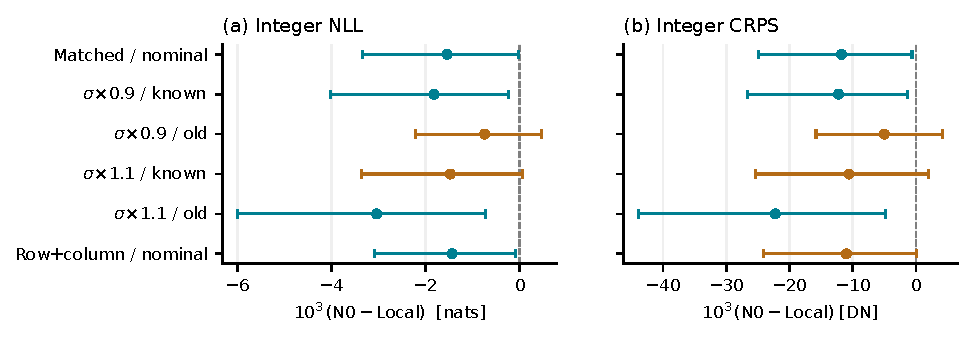
\includegraphics[width=\textwidth]{f09_paired_stress.pdf}
\caption{Paired calibration and correlation tests on 32 development sources. Each setting uses 8,192 central zero candidates shared by both methods. Points show mean differences averaged first over CFA phases and then over sources, with 95\% source-bootstrap intervals (negative values favor N0). The \emph{known} setting supplies the changed profile to both estimators and their decoders, whereas the \emph{old} setting retains the original calibration. Row and column offsets are unobserved, and orange intervals cross zero.}
\label{fig:pairedstress}
\end{figure*}

\section{Additional Development Controls}\label{sec:v3}
The post-hoc controls below use development data to complement the registered held-out test.

\subsection{Joint-CFA Local Development Comparator}
Joint-CFA local Bayes uses 256 equally weighted four-phase signal templates (two per scene from 128 training scenes), evaluates a packed $5\times5$ four-phase likelihood counting each censoring event once, and mixes the corresponding integer PG laws across 32,462 shared positions from 32 development sources.

\begin{table}[t]
\centering
\caption{Post-hoc development comparison on 32 fixed sources. CFA means are computed within source, followed by equal source weighting.}
\label{tab:joint}
\scriptsize
\setlength{\tabcolsep}{3pt}
\begin{tabular}{@{}lrrr@{}}
\toprule
Method & Excess KL & NLL & CRPS\\
& (nats) & (nats) & (DN)\\
\midrule
N0/PG & 0.000376673 & 3.911227506 & 8.103882756\\
Joint-CFA local Bayes & 0.001790969 & 3.912282251 & 8.112198163\\
Same-CFA Local PG & 0.001952344 & 3.912362493 & 8.112870272\\
\bottomrule
\end{tabular}
\end{table}

In Table~\ref{tab:joint}, the N0-minus-Joint-CFA differences and 95\% source-bootstrap intervals are $-0.00141430$ nats ($[-0.00296235,-0.00031761]$) for excess KL, $-0.00105475$ nats ($[-0.00215630,-0.00029750]$) for NLL, and $-0.00831541$ DN ($[-0.01755261,-0.00217521]$) for CRPS, whereas the Joint-CFA-minus-Local-PG NLL and CRPS intervals cross zero.

\subsection{Runtime and Resource Table}
\begin{table}[tbp]
\centering
\caption{In-memory implementation cost, excluding decoding, initialization, and file output. Backends and warm-up differ as specified in the text.}
\label{tab:runtime}
\footnotesize
\begin{tabular}{@{}lrr@{}}
\toprule
Metric & N0/PG & Local PG $3\times3$\\
\midrule
128 packed median (s) & 0.2074 & 0.7329\\
24MP median of 3 (s) & 27.3901 & 205.1503\\
24MP range (s) & 25.1087--27.9992 & 194.3892--219.9394\\
CUDA allocated (MiB) & 750.69 & 94.84\\
CUDA reserved (MiB) & 1112.00 & 254.00\\
\bottomrule
\end{tabular}
\end{table}

Table~\ref{tab:runtime} benchmarks an RTX 3090 Ti (Python 3.10, PyTorch 2.6/CUDA 12.4, two CPU threads, synchronized GPU stages) on a 24MP frame with 2,637,992 zeros. Patches use 10 warmup and 30 timed runs, while for 24MP frames N0 uses 10 warmup and 3 timed runs and Local PG combines one pilot with two subsequent runs. N0 uses FP32 GPU inference and GPU LUT interpolation, whereas Local PG uses FP64 GPU likelihoods and CPU LUT interpolation, and both sample on CPU. With a 128-pixel core and 1-pixel halo for tiled Local PG, signal error across 32 checked positions is below $3.05\times10^{-12}$ DN, LUT PMFs match, and tile MLEs remain at least 179.14 DN below the grid limit.

\subsection{Paired Calibration and Correlation Probes}
N0 and same-CFA $5\times5$ Local PG are evaluated on shared inputs from 32 development sources (128-pixel packed context, central 64-pixel region, at most 64 zeros per phase, averaged over phases and then sources with 10,000-resample 95\% intervals). At read-noise factors of $0.9$ and $1.1$, both methods receive either the true perturbed profile (extrapolating N0's constant channels beyond training) or the nominal old profile. Unobserved Gaussian row and column offsets (5 DN standard deviation each) omit oracle KL and resolve the integer PG tail.

In Fig.~\ref{fig:pairedstress}, old calibration at $0.9\sigma$ gives NLL $-0.000746$ nats ($[-0.002214,0.000462]$), and known $1.1\sigma$ is likewise inconclusive, whereas row and column offsets give NLL $-0.001439$ nats ($[-0.003090,-0.000090]$) while the CRPS interval crosses zero.

\subsection{Real-Code Event Scope}\label{sec:realcode}
All 31,852 primary real candidates are retained. The nested $V\leq-128$, $V\leq-256$, and $V\leq-305$ DN thresholds contain 122, 21, and 13 events, with the deepest 13 decoding to native 79--202 DN (aligned $-430$ to $-307$ DN). Two coordinates repeat below $-128$ DN (one below $-305$ DN), and the full frames separately contain 18 and 25 native zeros, while ten dark frames supply calibration. Although the deepest 13 events add 0.03917 and 0.04525 nats to absolute N0 NLL, they change the paired difference by only $+0.0000040$ and $-0.0000083$ nats, and removing $V\leq-128$ DN leaves NLL differences of $-0.001375$ and $-0.000998$ nats (Table~\ref{tab:real_robust}).

N0 has lower NLL in 7 of 12 fixed ROIs. Symmetric 1\% winsorization gives paired NLL differences of $-0.001269$ and $-0.001082$ nats (versus $-0.001342$ and $-0.000964$ for all events). Diagnostic B-phase NLL for N0 vs.\ Local PG is 3.807768 vs.\ 3.810883 and 3.857925 vs.\ 3.859954 nats in the two exposures.

\end{document}
